\documentclass[12pt]{article}


\usepackage{amssymb}
\usepackage{amsmath}
\usepackage{fullpage}
\usepackage{epsfig}
\usepackage{epstopdf}
\everymath{\displaystyle}
\usepackage{enumerate}

\newif\ifans

\anstrue

\begin{document}

\begin{center}
\underline{\LARGE{Chapter 1.1: Bisection (Interval Halving) Method}}
\end{center}

\subsection*{Expected Skills:}

\begin{itemize}

\item Be able to state the Intermediate Value Theorem and use it to prove the existence of a solution to $f(x)=0$ in an interval $(a,b)$.

\item Be able to apply the Bisection (Interval Halving) Method to approximate a solution to $f(x)=0$.

\item Be able to use different stopping procedures to exit the Bisection Method algorithm, as described in the notes.

\end{itemize}

\subsection*{Practice Problems: }

\begin{enumerate}

\item State the Intermediate Value Theorem.  What are the assumptions?  What are the conclusions?

\ifans {\fbox{\parbox{1\linewidth}{See the notes for the theorem's statement. There are two assumptions.  The first is that $f(x)$ is continuous on $[a,b]$.  The second is that $f(a)$ and $f(b)$ have different signs.  If these assumptions are satisfied, then the conclusion is that there must be at least one $x$ in the interval $(a,b)$ for which $f(x)=0$.}}} \fi

\item Sketch the graph of a function which satisfies the assumptions of the intermediate value theorem on the interval $[a,b]$ and which has:

\begin{enumerate}

\item Exactly one solution to $f(x)=0$ in the interval $(a,b)$.

\ifans{\fbox{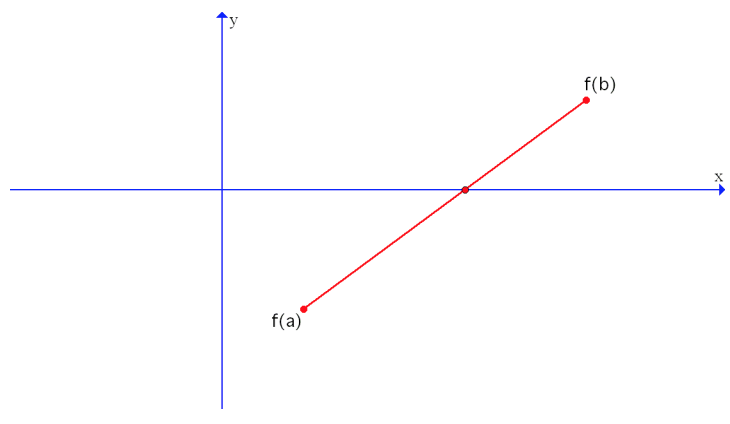
\includegraphics[scale=0.7]{graph3.png}}}\fi

\ifans{\newpage}\fi
\item Exactly two solutions to $f(x)=0$ in the interval $(a,b)$.

\ifans{\fbox{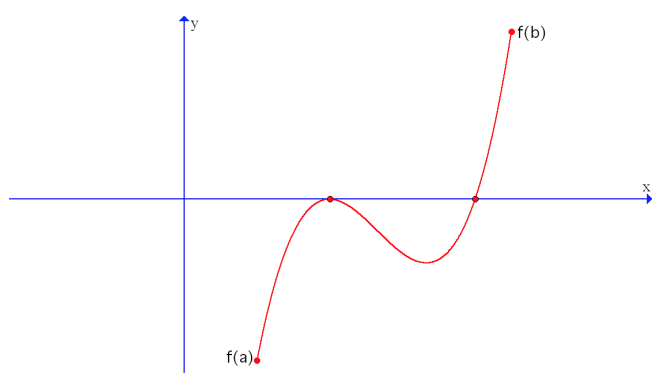
\includegraphics[scale=0.7]{graph2.png}}}\fi

\item Exactly three solutions to $f(x)=0$ in the interval $(a,b)$.

\ifans{\fbox{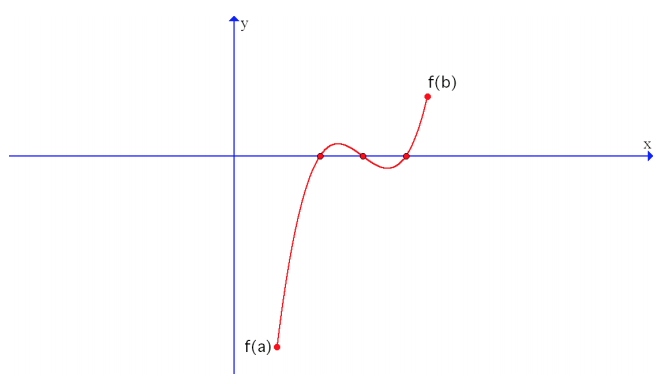
\includegraphics[scale=0.7]{graph1.png}}}\fi

\end{enumerate}

\item By appealing to the Intermediate Value Theorem, justify the existence of a solution to $x^5-7x+3=0$ in the interval $(1,2)$.

\ifans{\fbox{\parbox{1\linewidth}{Let $f(x)=x^5-7x+3$.  $f(x)$ is always continuous because it is a polynomial.  Thus, since $f(x)$ is continuous on $[1,3]$ with $f(1)=-3<0$ and $f(2)=21>0$, the intermediate value theorem guarantees at least one solution to $f(x)=0$ on  the interval $(1,2)$.}}} \fi

\item Use the Bisection Method to estimate a solution to $x^3+7x-5=0$ in the interval $(0,8)$ using the stopping procedures listed below.  In each case, what is an estimate of the desired solution?  How many iterations do you have to perform?

\begin{enumerate}

\item Use the stopping algorithm described in Algorithm 1.1.1 of the notes with $\epsilon=0.1$.

\ifans\fbox{The solution is approximately 0.6875 after 7 iterations.}\fi

\item Again let $\epsilon=0.1$.  Use the stopping algorithm: ``If $|f(m_k)|<\epsilon$, stop.  Else, perform another iteration."

\ifans\fbox{The solution is approximately 0.671875 after 9 iterations.}\fi

\item Again let $\epsilon=0.1$.  Use the stopping algorithm: ``If $|m_k-m_{k-1}|<\epsilon$, stop.  Else, perform another iteration."

\ifans\fbox{The solution is approximately 0.6875 after 7 iterations.}\fi

\end{enumerate}

\item Estimate $\sqrt{3}$ using the bisection method.  Initialize your search with $[a,b]=[0,2]$ and use the stopping procedures listed below.  In each case, what is the estimated value of $\sqrt{3}$ and how many iterations were required?  (Hint: find the positive value of $x$ such that $x^2=3$.)

\begin{enumerate}

\item Use the stopping algorithm described in Algorithm 1.1.1 of the notes with $\epsilon=0.1$.

\ifans\fbox{The solution is approximately 1.6875 after 5 iterations.}\fi

\item Again let $\epsilon=0.1$.  Use the stopping algorithm: ``If $|f(m_k)|<\epsilon$, stop.  Else, perform another iteration."

\ifans\fbox{The solution is approximately 1.75 after 3 iterations.}\fi

\item Again let $\epsilon=0.1$.  Use the stopping algorithm: ``If $|m_k-m_{k-1}|<\epsilon$, stop.  Else, perform another iteration."

\ifans\fbox{The solution is approximately 1.6875 after 5 iterations.}\fi

\end{enumerate}

\item The  {\bf False position (regula falsi)}, sometimes called linear interpolation method, is an iterative process designed to speed up the bisection method; it works to approximate a solution to $f(x)=0$, where $f(x)$ satisfies the same hypotheses of the bisection method.  Given two points $(a_n,f(a_n)$ and $(b_n,f(b_n))$ satisfying $f(a_n)f(b_n)<0$, the secant line which passes through both of these points will cross the $x$-axis, as in the figure below.
\begin{center}
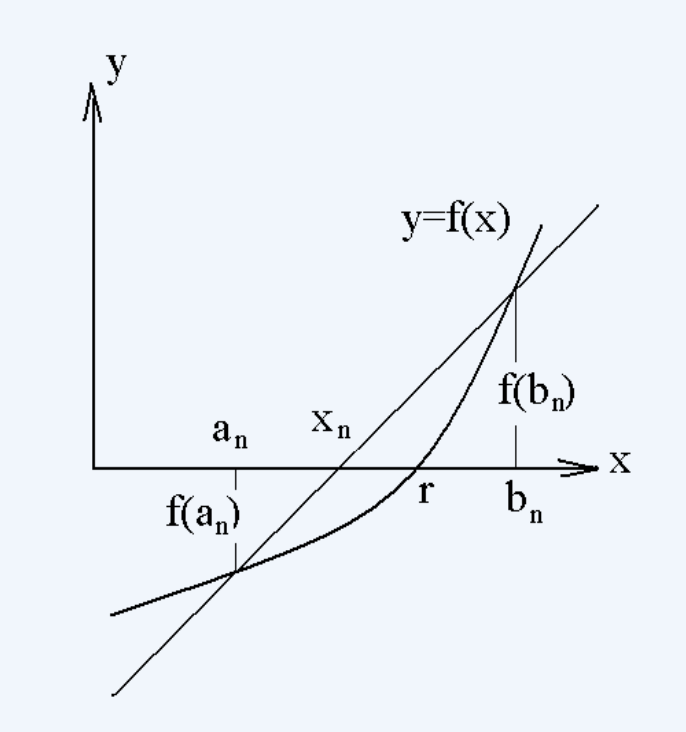
\includegraphics[scale=0.5]{LinearInterp.png}
\end{center}
In each iteration, rather than choosing the midpoint of the interval $(a_n,b_n)$ as the next approximation of the solution as is done in the bisection method, the update is chosen to be the $x$ intercept of this secant line.  Then, the algorithm would continue as in the bisection method.

Derive a formula for $x_n$, the approximation generated by the False position method when the current interval is $(a_n,b_n)$.

\ifans{\fbox{$x_{n} = a_n - \frac{f(a_n)(b_n-a_n)}{f(b_n)-f(a_n)}$}} \fi

\end{enumerate}

\end{document}